\mychapter{3}{Opis riešenia - Server manažmentu rolí a používateľov}


%ked vyhladavam užívateľov, nemal by som dať limit... aj ked to mi neotestujú :D
\section{Určenie požiadaviek}
Aplikačným výstupom tejto bakalárskej práce je web stránka, ktorej účelom je vytvoriť jednoduché a intuitívne aplikačné rozhranie pre priraďovanie používateľov k roliam. V aplikácii by sa mali dať vyhľadať všetci používatelia vo firme. Pre rýchlejšie vyhľadávanie a prehľadné údaje bude možné používateľov zotriediť do kategórie podľa rolí. Užívatelia, ktorí nemajú priradenú žiadnu rolu, budú mať vlastnú podsekciu. Vďaka tomu bude mať firma každého používateľa pod kontrolou, aby mal priradenú minimálne jednu rolu. Užívatelia sa budú dať zoradiť podľa ich id, mena, priezviska alebo e-mailovej adresy. V každej podsekcii umožníme vyhľadávať konkrétneho používateľa na základe textového vstupu. Vstup sa porovná s id,menom, priezviskom aj emailom každého používateľa z vybranej podsekcie. Niektoré firmy majú vo svojej štruktúre niekoľko desiatok zamestnancov.   Každý používateľ sa bude dať jednotne aj skupinovo priradiť k požadovanej role. Zároveň bude možné osobitne spravovať roly pre konkrétneho člena firmy. Ďalšou funkcionalitou aplikácie je manažment rol vo firme. Do firmy bude možné vložiť nové roly, prípadne niektoré roly odstrániť. Pri odstránení roly z firmy, treba dať pozor, aby sme nemohli odstrániť roly, ktoré firma práve používa na vykonávanie vlastných procesov. Takýmto spôsobom bude možné do firmy pridať roly z xml súboru vygenerované v aplikácii na vytváranie a prideľovanie rolí k procesom od Kristiána Stroku. Túto funkcionalitu bude možné pri integrácii plne odstrániť. Zároveň má aplikácia poskytovať rozhranie, prostredníctvom ktorého  bude možné výstup od Kristiána Stroku možné uložiť do databázy. 


\section{Implementácia}
V tejto časti sa zameriame na podrobný opis implementácie modulu na správu a priraďovanie rolí k používateľom. Podrobne si vysvetlíme fungovanie rolí v systéme, vysvetlíme databázový model a popíšeme celkovú architektúru a spôsob implementácie rolí v našom systéme. Rozoberieme možné bezpečnostné riziká a spôsob ich riešenia.

\subsection{Popis architektúry}
Základnou myšlienkou RBAC architektúry je odstrániť priame priraďovanie práv k používateľom. Tento výsledok sa zabezpečí pridaním medzikroku a teda rolí medzi samotných používateľov a ich právomoci .Samotná implementácia tejto architektúry závisí od konkrétneho systému a jeho architektúry. Naša aplikácia sa zameriava na vytvorenie WfMS za pomoci Petriho sietí. Ako prvé si definujeme základnú architektúru. Na Obr. \ref{fig:model_rbac_v_aplikacii} môžeme zreteľne vidieť dve nezávislé časti fungovania workflow systému. V ľavej časti ilustrácie vidíme sekciu, ktorá sa zaoberá  prideľovaním  používateľou k roliam, zatiaľ čo pravá časť znázorňuje proces samotný. Vo firme je vďaka tomu zabezpečené, aby sa procesy mohli vytvárať nezávisle od používateľov. Priraďovanie práv je zabezpečené väzbou medzi rolami a procesmi. Pre správnu funkcionalitu je však potrebné, aby firma mala priradené tie role, ktoré sú použité v jednotlivých procesoch, ktoré firma využíva. Definovanie prístupových práv je zabezpečené nad samotnými prechodmi v sieti.

\begin{figure}[h]
	\centering
	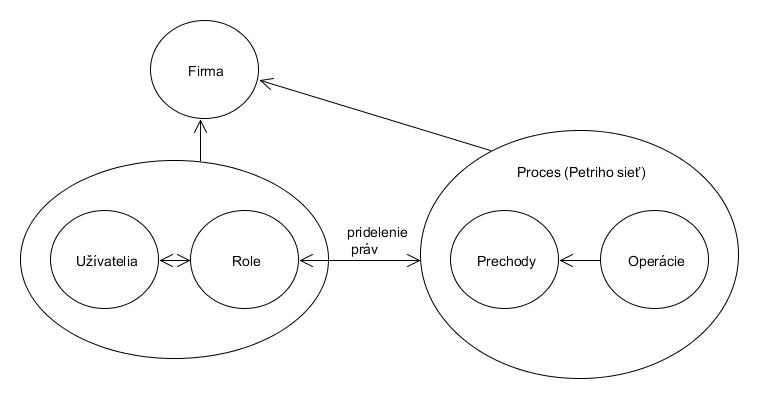
\includegraphics[width=0.9\linewidth]{images/roles_in_petri_model}
	\caption{ Model RBAC v aplikácii}
	\label{fig:model_rbac_v_aplikacii}
\end{figure}

\subsection{Priraďovanie používateľov k roliam}
V našej aplikácii nechceme aby bol používateľ viazaný len na jednu firmu. Chceme aby pod rovnakým účtom mohol figurovať vo viacerých firmách, prípadne mal možnosť si založiť vlastnú. Preto je potrebné, aby sa používatelia neviazali len na samotnú rolu. V aplikácii bude väzba používateľa na rolu závislá od konkrétnej firmy. V každej firme bude môcť administrátor, používateľ s právami na riadenie rolí, mať možnosť priradiť používateľa ku konkrétnej role, ktorá je vo firme obsiahnutá. Samotný používateľ môže byť tým pádom priradený vo viacerých firmách, pričom v každej firme bude mať iné práva. Na obrázku  \ref{fig:user_to_roles} môžeme vidieť zjednodušený model mapovania právomocí používateľa prostredníctvom systému rolí.
Šedé pozadie v roli znamená, že používateľ je k roli priradený.  V rovnakom procese vidíme, že používateľ, ktorý môže vo firme 1 spustiť prechod 1 , nie je oprávnený vykonať prechod 1 aj vo firme 2, pretože v nej nemá priradenú rolu. Vo firme 2 môže spustiť iba prechod 2.

\begin{figure}[h]
	\centering
	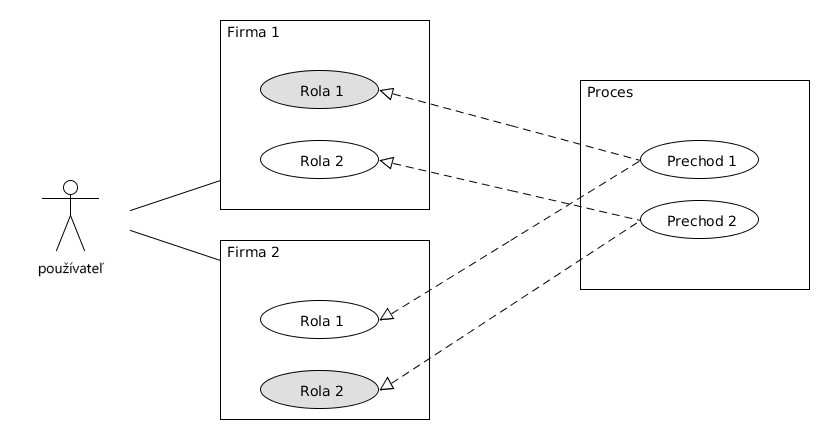
\includegraphics[width=0.9\linewidth]{images/user_to_roles}
	\caption{ Model RBAC v aplikácii}
	\label{fig:user_to_roles}
\end{figure}


\subsection{Riadenie právomocí}	
Zadefinovali sme si ako sa v aplikácii mapujú používatelia na role. V nasledujúcej časti si bližšie definujeme pravidlá pre spúšťanie prechodov v sieti, rovnako ako aj samotné právomoci ktoré daná rola v procese nadobudne. 



\subsubsection{Priradenie práv k roliam}
Priradenie práv k roliam je definované nepriamo prostredníctvom jednotlivých prechodov. Hlavnou úlohou role v procese je zadefinovať práva na vytváranie nových prípadov a takisto určiť právomoci na spúšťanie prechodov v procese. Schopnosť spustiť nový prechod je však vymedzená referenciami, návrhom Petriho siete a stave v akom sa tokeny momentálne nachádzajú.  


\begin{figure}[h]
	\centering
	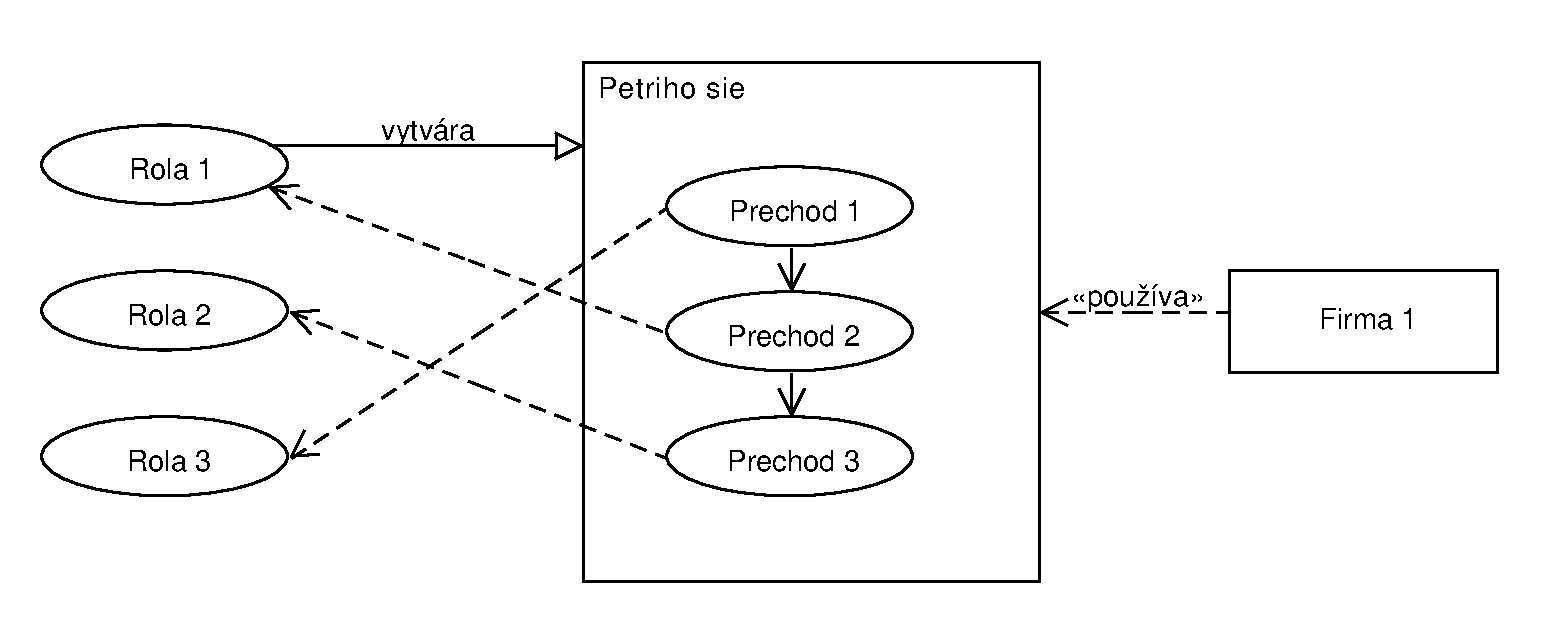
\includegraphics[width=0.9\linewidth]{images/roles_permissions}
	\caption{ Právomoci rolí v sieti }
	\label{fig:roles_permissions}
\end{figure}

\subsubsection{Definovanie prístupových práv ku prechodu}

Osoba môže v jednotlivom prípade spustiť prechod, ak spĺňa nasledovné požiadavky:
\begin{enumerate}
	\item prechod je spustiteľný
	\item osoba je priradená k roli, ktorej daný prechod prináleží
	\item osoba spľňa požiadavky referencie
\end{enumerate}

Spustiteľnosť prechodu je zadefinovaná prostredníctvom Petriho siete. Prechod v sieti je spustiteľný len vtedy, ak každé  miesto vstupujúce do prechodu obsahuje minimálne toľko tokenov, aká je násobnosť hrany medzi daným miestom a prechodom.
V aplikácii máme dva typy referencii: \textbf{referenciu na prechod} a \textbf{referenciu na prvú rolu} .
Ak má prechod nastavenú referenciu na prechod, v databáze sa porovná používateľove id s id používateľa , ktorý spustil referovaný prechod. V prípade, že tieto dáta súhlasia, používateľ je oprávnený spustiť prechod.

Ak má prechod nastavenú referenciu na prvého používateľa, overí sa ,či sa v procese už daná rola nevyskytla. Ak prechod s danou rolou v danom prípade ešte nebol spustený, používateľ je oprávnený tento prechod spustiť. V opačnom prípade je potrebné overiť id používateľa s používateľom ktorý ako prvý spustil prechod s touto rolou. Ak sa zistí zhoda, používateľ môže daný prechod spustiť.



\subsubsection{Operácie nad prechodom}	
Práva, ktoré rola nad prechodom získa sú zadefinované operáciami v konkrétnom prechode. Tieto operácie sa určia pri vytváraní formulára k danému prechodu.  
Vo formulári je možné nastaviť aké dáta budú používateľovi prístupné, či ich bude môcť používateľ iba zobrazovať, alebo aj editovať. Takisto sa definuje, ktoré údaje je potrebné vyplniť, aby mohol používateľ tento prechod dokončiť.


\subsection{Datový model}
Dátová časť našej aplikácie je implementovaná v databáze MySQL5.1. Na začiatku je potrebné definovať návrh tabuliek pre uloženie rolí a referencii ku konkrétnej sieti. Druhým krokom je návrh databázového modelu, ktorý bude umožňovať konkrétnym používateľom vo firme priradiť rolu.
Pre tieto účely sme si definovali nasledovné tabuľky:
ROLES,TRANSITIONS\_X\_ROLE , ROLES\_START\_CASES, REFERENCES, USERS, USERS\_X\_FIRM, USERS\_X\_ROLE 
Do tabuľky ROLES budeme ukladať role a ich názov. Názov role sme zvolili ako unikátny atribút, kvôli tomu aby bolo uľahčené ukladanie role do databázy. TODOOOOO . V tabuľke TRANSITIONS\_X\_ROLE sa viažu role na prechody v petriho sieti. Každý prechod bude mať v tejto tabuľke presne určené , ktorá roľa ho môže spustiť. V Tabuľke ROLES\_START\_CASES priradíme k petriho sieti rolu, ktorá môže spustiť nový prípad. V tabuľke REFERENCES definujeme , či má prechod v sieti referenciu. Atribút  value typu boolean v tejto tabuľke definuje, či má prechod referenciu. Ak má referenciu, v atribúte referenced\_transition\_id sa skontroluje,či obsahuje referenciu na konkrétny prechod. V prípade , že tento atribút nemá hodnotu NULL, odkazuje tento atribút na primárny kľúč referencovaného prechodu. V tabuľke USERS budú uložený jednotlivý používatelia, ich prihlasovacie a osobné údaje. V tabuľke USERS\_X\_FIRM priraďujeme používateľov ku firmám a v tabuľke USERS\_X\_ROLE priraďujeme používateľom role v jednotlivých firmách. V tejto tabuľke sme zvolili ako primárny kľúč kombináciu cudzích kľúčov odkazujúcich na id používateľa, role a firmy . 



\subsection{Ukladanie rolí a referencii k Petriho sieti}




\subsection{Používateľské rozhranie}



\section{Overenie riešenia}
TODO